\documentclass[notitlepage]{ctexrep}
\usepackage{amsmath,amsfonts,amsthm,amssymb}
\usepackage{authblk}
\usepackage[T1]{fontenc}
\usepackage{graphicx}
\usepackage[utf8]{inputenc}
\usepackage[framemethod=tikz]{mdframed}
\usepackage{natbib}
\usepackage{subcaption}
\usepackage{tikz}
\usepackage{xcolor}
\usepackage{epigraph}
\usepackage{float}


%设置超链接
\usepackage[colorlinks,linkcolor=blue,
citecolor=red]{hyperref}


\definecolor{blue}{RGB}{38,139,210}
\definecolor{cyan}{RGB}{42,161,152}
\definecolor{violet}{RGB}{108,113,196}
\definecolor{red}{RGB}{220,50,47}
\definecolor{base01}{RGB}{88,110,117}
\definecolor{base02}{RGB}{7,54,66}
\definecolor{base03}{RGB}{0,43,54}

\usetikzlibrary{calc,shapes,positioning}

\newcommand{\todo}[1]{\textcolor{red}{TODO: #1}}

\newtheorem{relationship}{关系}
\providecommand*{\relationshipautorefname}{关系}
\surroundwithmdframed[
    topline=false,
    bottomline=false,
    middlelinewidth=0.5pt,
    linecolor=base01,
    roundcorner=5pt,
    innertopmargin=0pt,
    leftmargin=15pt,
    rightmargin=15pt,
    nobreak=true,
]{relationship}

\setcounter{MaxMatrixCols}{16}

\let\originalepigraph\epigraph
\renewcommand\epigraph[2]{\originalepigraph{\textit{#1}}{\textsc{#2}}}

% Use arabic numbers for thanks
\makeatletter
\let\@fnsymbol\@arabic
\makeatother

\title{A guide to convolution arithmetic for deep learning}
\author[$\bigstar$]{Vincent Dumoulin\thanks{dumouliv@iro.umontreal.ca}}
\author[$\bigstar\dagger$]{Francesco Visin\thanks{francesco.visin@polimi.it}}
\affil[$\bigstar$]{MILA, Universit\'{e} de Montr\'{e}al}
\affil[$\dagger$]{AIRLab, Politecnico di Milano}
\date{2018.1.12}

\begin{document}

\maketitle
\thispagestyle{empty}
\clearpage

\setlength{\epigraphwidth}{0.4\textwidth}
\epigraph{All models are wrong, but some are useful.}{George E. P. Box}
\clearpage

\renewcommand{\abstractname}{Acknowledgements}
\begin{abstract}
    The authors of this guide would like to thank David Warde-Farley, Guillaume
    Alain and Caglar Gulcehre for their valuable feedback. We are likewise
    grateful to all those who helped improve this tutorial with helpful
    comments, constructive criticisms and code contributions. Keep them coming!

    Special thanks to Ethan Schoonover, creator of the Solarized color
    scheme,\footnote{\url{http://ethanschoonover.com/solarized}} whose colors
    were used for the figures.
\end{abstract}

\renewcommand{\abstractname}{Feedback}
\begin{abstract}
    Your feedback is welcomed! We did our best to be as precise, informative and
    up to the point as possible, but should there be anything you feel might be
    an error or could be rephrased to be more precise or comprehensible, please
    don't refrain from contacting us. Likewise, drop us a line if you think
    there is something that might fit this technical report and you would like
    us to discuss -- we will make our best effort to update this document.
\end{abstract}

\renewcommand{\abstractname}{Source code and animations}
\begin{abstract}
    The code used to generate this guide along with its figures is available on
    GitHub.\footnote{\url{https://github.com/vdumoulin/conv_arithmetic}} There
    the reader can also find an animated version of the figures.
\end{abstract}

\tableofcontents

\chapter{引言}

深度卷积神经网络 (CNNs) 一直是深度学习取得巨大进步的核心. 尽管卷积神经网络在九十年代就被用来解决字符识别任务\citep{le1997reading},它们当前的广泛应用是由于最近的工作,当时一个深层CNN被用来打败最先进的ImageNet图像分类挑战\citep{krizhevsky2012imagenet}.

因此卷积神经网络为机器学习的专业人士构建了一个非常有用的工具. 然而,第一次学习使用卷积神经网络通常是一种``可怕''的经历. 一个卷积层的输出形状受它的输入形状及卷积核的形状、零填充和步长的选择所影响,并且这些特性之间的关系不可忽视. 这不同于输出尺寸依赖于输入尺寸的全连接层. 另外,卷积神经网络通常还具有一个 {\em
池化\/}(pooling) 阶段,对全连接网络来说增加了另一层的复杂性. 最后,所谓的转置卷积层(也被称为分步卷积层)近期已经在越来越多的工作\citep{zeiler2011adaptive,zeiler2014visualizing,
long2015fully,radford2015unsupervised,visin15,im2016generating}, 中被采用,并且它们与卷积层的关系已经从多个角度解释清楚了. 

本指南的目标有两个:

\begin{enumerate}
    \item 解释卷积层和转置卷积层.
    \item 直观地理解卷积、池化和转置卷积层中输入形状、卷积核形状、零填充、步长和输出形状之间的关系. 
\end{enumerate}

为了保持普适性,本指南中所示结果不依赖实现细节,并适用于所有常用的机器学习框架,例如Theano
\citep{bergstra2010theano,bastien2012theano}, Torch \citep{collobert2011torch7},
Tensorflow \citep{abaditensorflow} 和 Caffe \citep{jia2014caffe}.

本章简要回顾卷积神经网络的主要组成部分,即离散卷积和池化. 为了深入研究这一问题,请看深度学习教材的第九章\citep{Goodfellow-et-al-2016-Book}.

\section{离散卷积}

神经网络的中心思想是 \emph{仿射变换}(affine transformations): 一个向量被接收为输入(input),并与矩阵相乘以产生输出(在进行非线性传递之前,通常会添加一个偏置向量). 这适用于任何类型的输入,无论是图像、音频片段还是无序的特征集合:无论它们的维数如何,在变换之前,它们的表示都可以被展成向量.

图像、音频片段和许多其他相似类型的数据都有一个本质的结构. 从形式上讲,它们共享这些重要的性质:

\begin{itemize}
    \item 它们被存储为多维数组.
    \item 它们以一个或多个轴为特征,它们之间的顺序很重要(例如,图像的宽度和高度轴,音频片段的时间轴)。
    \item 一个轴称为通道轴 (channel axis),用于访问数据的不同视图(例如,彩色图像的红色,绿色和蓝色通道,或立体声音频轨道的左右通道)。 
\end{itemize}

在应用仿射变换之前,这些性质还未被利用;事实上,所有的轴都以相同的方式处理,而且没有考虑拓扑的信息. 尽管如此,利用数据的隐式结构可能在完成某些任务,如计算机视觉和语义识别时非常方便,在这些情况下最好保存这些数据. 这就是离散卷积发挥作用的地方. 

离散卷积是一种线性变换,它保留了顺序的概念. 离散卷积是稀疏的(只有几个输入单元对给定的输出单元有贡献),并且重用参数(相同的权重应用于输入的多个位置). 

\autoref{fig:numerical_no_padding_no_strides} 给出了一个离散卷积的例子. 浅蓝色的网格称为 {\em 输入特征映射} (input feature map). 为了保持绘图的简洁,该图代表了一个输入特征映射,但多个特征映射一个置于另一个上也很常见. \footnote{%
    在这方面的一个例子就是之前提到的图像和音频片段 {\em 通道\/} (channels) .} {\em 卷积核\/} (阴影区域)在输入特征映射中滑动. 在每个位置,计算卷积核的每个元素与它重叠的输入元素之间的乘积,

\begin{figure}[H]
    \centering
    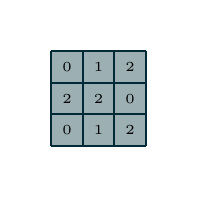
\begin{tikzpicture}[scale=.4,every node/.style={minimum size=1cm}, on grid]
            \draw[fill=base02,opacity=0.4] (0,0) rectangle (3,3);
            \draw[draw=base03,thick] (0,0) grid (3,3);
            \node (00) at (0.5,2.5) {\tiny 0};
            \node (01) at (1.5,2.5) {\tiny 1};
            \node (02) at (2.5,2.5) {\tiny 2};
            \node (10) at (0.5,1.5) {\tiny 2};
            \node (11) at (1.5,1.5) {\tiny 2};
            \node (12) at (2.5,1.5) {\tiny 0};
            \node (20) at (0.5,0.5) {\tiny 0};
            \node (21) at (1.5,0.5) {\tiny 1};
            \node (22) at (2.5,0.5) {\tiny 2};
    \end{tikzpicture}
\end{figure}

\begin{figure}[p]
    \centering
    \includegraphics[width=0.32\textwidth]{pdf/numerical_no_padding_no_strides_00.pdf}
    \includegraphics[width=0.32\textwidth]{pdf/numerical_no_padding_no_strides_01.pdf}
    \includegraphics[width=0.32\textwidth]{pdf/numerical_no_padding_no_strides_02.pdf}
    \includegraphics[width=0.32\textwidth]{pdf/numerical_no_padding_no_strides_03.pdf}
    \includegraphics[width=0.32\textwidth]{pdf/numerical_no_padding_no_strides_04.pdf}
    \includegraphics[width=0.32\textwidth]{pdf/numerical_no_padding_no_strides_05.pdf}
    \includegraphics[width=0.32\textwidth]{pdf/numerical_no_padding_no_strides_06.pdf}
    \includegraphics[width=0.32\textwidth]{pdf/numerical_no_padding_no_strides_07.pdf}
    \includegraphics[width=0.32\textwidth]{pdf/numerical_no_padding_no_strides_08.pdf}
    \caption{\label{fig:numerical_no_padding_no_strides} 计算离散卷积的输出值.}
\end{figure}

\begin{figure}[p]
    \centering
    \includegraphics[width=0.32\textwidth]{pdf/numerical_padding_strides_00.pdf}
    \includegraphics[width=0.32\textwidth]{pdf/numerical_padding_strides_01.pdf}
    \includegraphics[width=0.32\textwidth]{pdf/numerical_padding_strides_02.pdf}
    \includegraphics[width=0.32\textwidth]{pdf/numerical_padding_strides_03.pdf}
    \includegraphics[width=0.32\textwidth]{pdf/numerical_padding_strides_04.pdf}
    \includegraphics[width=0.32\textwidth]{pdf/numerical_padding_strides_05.pdf}
    \includegraphics[width=0.32\textwidth]{pdf/numerical_padding_strides_06.pdf}
    \includegraphics[width=0.32\textwidth]{pdf/numerical_padding_strides_07.pdf}
    \includegraphics[width=0.32\textwidth]{pdf/numerical_padding_strides_08.pdf}
    \caption{\label{fig:numerical_padding_strides} 对 $N = 2$, $i_1 = i_2 = 5$, $k_1 = k_2 = 3$, $s_1 = s_2 = 2$, 和 $p_1 = p_2 = 1$ 计算离散卷积的输出值.}
\end{figure}


\noindent 并对结果进行求和. 可以用不同的卷积核重复该过程,以生成所需的输出特征映射  (\autoref{fig:full_picture}). 这个过程的最终输出被称为 {\em 输出特征映射} (output feature maps). \footnote{%
    虽然从信号处理的角度来看,卷积和交叉相关是有区别的,但当学习了卷积核时,两者就可以互换了. 为了简单起见,以及与大多数机器学习文献保持一致,我们将在这个指南中使用 {\em 卷积\/}(convolution) 这一术语.}

如果有多个输入特征映射,则核必须是三维的——或者等价于每个特征映射都用一个不同的核进行卷积,并且生成的特征映射主元素相加,以生成输出特征映射。

卷积(见图\autoref{fig:numerical_no_padding_no_strides})是二维卷积的一种形式,但是它可以生成N维卷积. 例如,在三维卷积中,卷积核可以是一个{\em 立方体\/} (cuboid),而且会在输入特征映射的的高度、宽度和深度上滑动. 

定义了一批离散卷积的核有一个形状对应$(n, m, k_1, \ldots, k_N)$的某个排列,其中

\begin{equation*}
\begin{split}
    n &\equiv \text{输出特征映射的数量},\\
    m &\equiv \text{输入特征映射的数量},\\
    k_j &\equiv \text{沿 $j$ 轴核的尺寸}.
\end{split}
\end{equation*}

以下属性会影响沿$j$轴方向卷积层的输出尺寸$o_j$ : 
\begin{itemize}
    \item $i_j$: 沿 $j$轴的输入尺寸,
    \item $k_j$: 沿 $j$轴的核尺寸,
    \item $s_j$: 沿$j$轴的步长 (核的两个连续位置之间的距离),
    \item $p_j$: 沿$j$轴方向的零填充 (在轴开始和结尾处连接的$0$的数目).
\end{itemize}

\noindent 例如, \autoref{fig:numerical_padding_strides} 展示了一个应用于$5 \times 5$输入的 $3
\times 3$ 卷积核,使用了 $2 \times 2$ 的步长填充了$1\times 1$的零边界.

注意,步长构成了一种 \emph{子采样}(subsampling) 形式. 步长作为衡量核被翻译多少的一种替代方法,它也可以看作保留了多少输出. 例如,以两个跃点移动卷积核相当于以一个跃点移动卷积核,但只保留奇数个输出元素 (\autoref{fig:strides_subsampling}).

\begin{figure}[p]
    \centering
    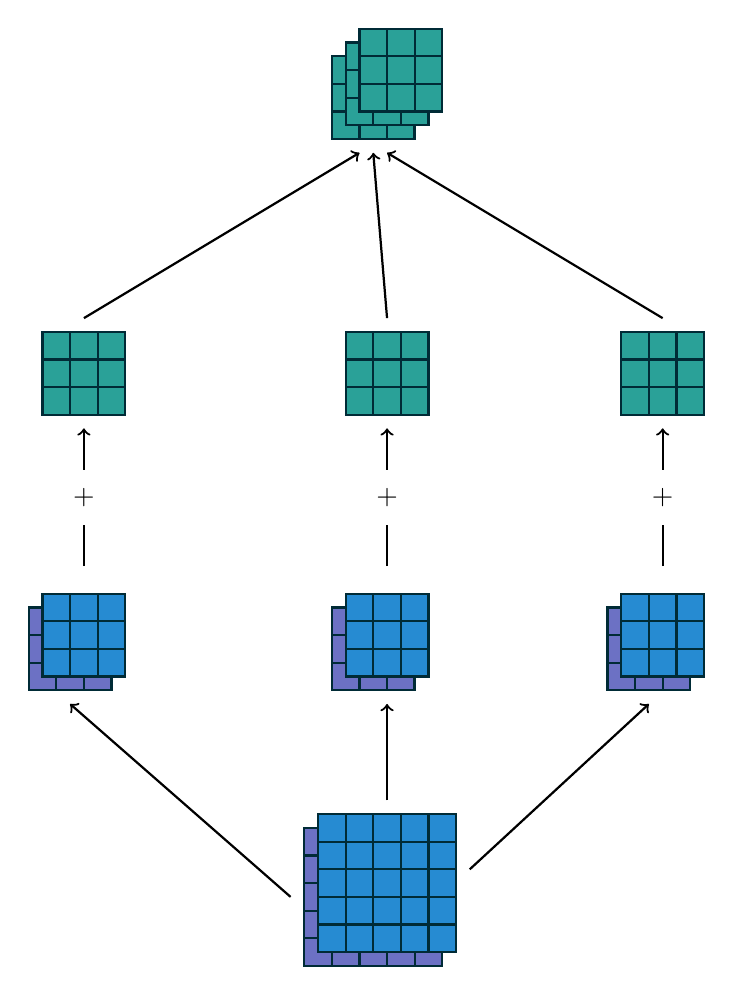
\begin{tikzpicture}[scale=.35,every node/.style={minimum size=1cm}, on grid]
        \begin{scope}[xshift=0cm,yshift=0cm]
            \begin{scope}[xshift=0cm,yshift=0cm]
                \draw[draw=base03,fill=violet,thick]
                    (0,0) grid (5,5) rectangle (0,0);
            \end{scope}
            \begin{scope}[xshift=0.5cm,yshift=0.5cm]
                \draw[draw=base03,fill=blue,thick]
                    (0,0) grid (5,5) rectangle (0,0);
            \end{scope}
        \end{scope}
        \foreach \x in {-10,1,11} {%
            \begin{scope}[xshift=\x cm,yshift=10cm]
                \begin{scope}[xshift=0cm,yshift=0cm]
                    \draw[draw=base03,fill=violet,thick]
                        (0,0) grid (3,3) rectangle (0,0);
                \end{scope}
                \begin{scope}[xshift=0.5cm,yshift=0.5cm]
                    \draw[draw=base03,fill=blue,thick]
                        (0,0) grid (3,3) rectangle (0,0);
                \end{scope}
            \end{scope}
            \begin{scope}[xshift=\x cm,yshift=20cm]\begin{scope}[xshift=0.5cm]
                \draw[draw=base03,fill=cyan,thick]
                    (0,0) grid (3,3) rectangle (0,0);
            \end{scope}\end{scope}
        }
        \begin{scope}[xshift=1cm,yshift=30cm]
            \foreach \s in {0.0,0.5,1.0} {%
                \begin{scope}[xshift=\s cm,yshift=\s cm]
                    \draw[draw=base03,fill=cyan,thick]
                        (0,0) grid (3,3) rectangle (0,0);
                \end{scope}
            }
        \end{scope}
        \draw[->, thick] (-0.5,2.5) to (-8.5,9.5);
        \draw[->, thick] (3,6) to (3,9.5);
        \draw[->, thick] (6,3.5) to (12.5,9.5);
        \draw[thick]  (-8,14.5) to (-8,16);
        \draw[->, thick]  (-8,18) to (-8,19.5);
        \node[thick] (p1) at (-8,17) {$+$};
        \draw[thick]  (3,14.5) to (3,16);
        \draw[->, thick]  (3,18) to (3,19.5);
        \node[thick] (p2) at (3,17) {$+$};
        \draw[thick]  (13,14.5) to (13,16);
        \draw[->, thick]  (13,18) to (13,19.5);
        \node[thick] (p3) at (13,17) {$+$};
        \draw[->, thick]  (-8,23.5) to (2,29.5);
        \draw[->, thick]  (3,23.5) to (2.5,29.5);
        \draw[->, thick]  (13,23.5) to (3,29.5);
    \end{tikzpicture}
    \caption{\label{fig:full_picture} 一种从两个输入特征映射到三个输出特征映射的卷积映射,使用$3 \times 2 \times 3 \times 3$的一批卷积核$\mathbf{w}$. 在左边的路径中,输入特征映射 1 与核 $\mathbf{w}_{1,1}$ 做卷积且输入特征映射 2 与核 $\mathbf{w}_{1,2}$做卷积,并将结果逐元素相加,形成第一个输出特征映射. 对中间和右侧的路径重复相同的步骤,以形成第二和第三个特征映射,并将所有的三个输出特征映射组合在一起形成输出.}
\end{figure}

\begin{figure}[p]
    \centering
    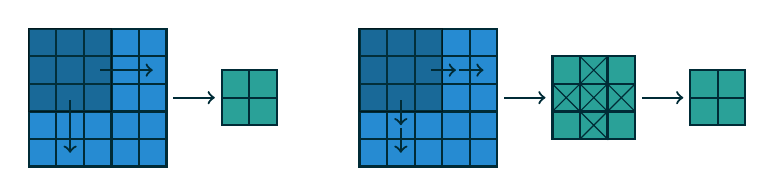
\begin{tikzpicture}[scale=.35,every node/.style={minimum size=1cm}, on grid]
        \begin{scope}[xshift=0,yshift=0cm]
            \begin{scope}[xshift=0cm,yshift=0cm]
                \draw[draw=base03,fill=blue,thick] (0,0) grid (5,5) rectangle (0,0);
                \draw[fill=base02, opacity=0.4] (0,2) rectangle (3,5);
            \end{scope}
            \begin{scope}[xshift=7cm,yshift=1.5cm]
                \draw[draw=base03,fill=cyan,thick] (0,0) grid (2,2) rectangle (0,0);
            \end{scope}
        \end{scope}
        \draw[draw=base03, ->, thick] (2.6,3.5) to  (4.5,3.5);
        \draw[draw=base03, ->, thick] (1.5,2.4) to (1.5,0.5);
        \draw[draw=base03, ->, thick] (5.25, 2.5) to (6.75, 2.5);
        \begin{scope}[xshift=12cm,yshift=0cm]
            \begin{scope}[xshift=0cm,yshift=0cm]
                \draw[draw=base03,fill=blue,thick] (0,0) grid (5,5) rectangle (0,0);
                \draw[fill=base02, opacity=0.4] (0,2) rectangle (3,5);
            \end{scope}
            \begin{scope}[xshift=7cm,yshift=1cm]
                \draw[draw=base03,fill=cyan,thick] (0,0) grid (3,3) rectangle (0,0);
                \draw[draw=base03] (1,0) -- (2,1) -- (2,0) -- (1,1);
                \draw[draw=base03] (0,1) -- (1,2) -- (1,1) -- (0,2);
                \draw[draw=base03] (1,1) -- (2,2) -- (2,1) -- (1,2);
                \draw[draw=base03] (2,1) -- (3,2) -- (3,1) -- (2,2);
                \draw[draw=base03] (1,2) -- (2,3) -- (2,2) -- (1,3);
            \end{scope}
            \begin{scope}[xshift=12cm,yshift=1.5cm]
                \draw[draw=base03,fill=cyan,thick] (0,0) grid (2,2) rectangle (0,0);
            \end{scope}
        \end{scope}
        \draw[draw=base03, ->, thick] (14.6,3.5) to  (15.5,3.5);
        \draw[draw=base03, ->, thick] (15.6,3.5) to  (16.5,3.5);
        \draw[draw=base03, ->, thick] (13.5,2.4) to (13.5,1.5);
        \draw[draw=base03, ->, thick] (13.5,1.4) to (13.5,0.5);
        \draw[draw=base03, ->, thick] (17.25, 2.5) to (18.75, 2.5);
        \draw[draw=base03, ->, thick] (22.25, 2.5) to (23.75, 2.5);
    \end{tikzpicture}
    \caption{\label{fig:strides_subsampling} 另一种步长可视方法. 不是以$s = 2$ (左边)的增量去转换 $3 \times 3$ 的卷积核,而是以 $1$ 为增量进行转换,且只保留一个 $s = 2$ 的输出元素(右边).}
\end{figure}

\section{池化}

除了离散卷积本身, {\em 池化\/} (pooling) 操作是构成卷积神经网络的另一个重要部分. 池化操作通过使用某种函数来汇总子区域,例如取平均值或最大值,以此减少特征映射的大小.

池化的工作原理是在输入中滑动一个窗口,并将窗口的内容提供给 {\em 池化函数} (pooling function). 从某种意义上讲,池化的工作原理与离散卷积十分类似,但它用其他函数代替了卷积核形成的线性组合. \autoref{fig:numerical_average_pooling}
给出了一个平均池化的例子, 而 \autoref{fig:numerical_max_pooling}
给出了最大值池化的例子.

以下属性会影响沿$j$轴池化层的输出大小$o_j$: 

\begin{itemize}
    \item $i_j$: 沿$j$轴的输入尺寸,
    \item $k_j$: 沿$j$轴的池化窗口大小,
    \item $s_j$: 沿$j$轴的步长 (池化窗口的两连续位置之间的距离).
\end{itemize}

\begin{figure}[p]
    \centering
    \includegraphics[width=0.32\textwidth]{pdf/numerical_average_pooling_00.pdf}
    \includegraphics[width=0.32\textwidth]{pdf/numerical_average_pooling_01.pdf}
    \includegraphics[width=0.32\textwidth]{pdf/numerical_average_pooling_02.pdf}
    \includegraphics[width=0.32\textwidth]{pdf/numerical_average_pooling_03.pdf}
    \includegraphics[width=0.32\textwidth]{pdf/numerical_average_pooling_04.pdf}
    \includegraphics[width=0.32\textwidth]{pdf/numerical_average_pooling_05.pdf}
    \includegraphics[width=0.32\textwidth]{pdf/numerical_average_pooling_06.pdf}
    \includegraphics[width=0.32\textwidth]{pdf/numerical_average_pooling_07.pdf}
    \includegraphics[width=0.32\textwidth]{pdf/numerical_average_pooling_08.pdf}
    \caption{\label{fig:numerical_average_pooling} 使用$1 \times 1$步长计算$5 \times 5$输入、$3 \times 3$平均池化操作的输出值.}
\end{figure}

\begin{figure}[p]
    \centering
    \includegraphics[width=0.32\textwidth]{pdf/numerical_max_pooling_00.pdf}
    \includegraphics[width=0.32\textwidth]{pdf/numerical_max_pooling_01.pdf}
    \includegraphics[width=0.32\textwidth]{pdf/numerical_max_pooling_02.pdf}
    \includegraphics[width=0.32\textwidth]{pdf/numerical_max_pooling_03.pdf}
    \includegraphics[width=0.32\textwidth]{pdf/numerical_max_pooling_04.pdf}
    \includegraphics[width=0.32\textwidth]{pdf/numerical_max_pooling_05.pdf}
    \includegraphics[width=0.32\textwidth]{pdf/numerical_max_pooling_06.pdf}
    \includegraphics[width=0.32\textwidth]{pdf/numerical_max_pooling_07.pdf}
    \includegraphics[width=0.32\textwidth]{pdf/numerical_max_pooling_08.pdf}
    \caption{\label{fig:numerical_max_pooling} 使用$1 \times 1$步长计算$5 \times 5$输入、$3 \times 3$最大值池化操作的输出值.}
\end{figure}

\chapter{卷积运算(Convolution arithmetic)}

卷积层属性之间的关系分析起来很容易,因为它们不跨轴交互,即沿$j$轴选定的卷积核大小、步长和零填充只影响$j$轴的输出大小. 因此,本章将重点介绍以下的简化设置:

\begin{itemize}
    \item 二维离散卷积 ($N = 2$),
    \item 方形输入 ($i_1 = i_2 = i$),
    \item 方形核尺寸 ($k_1 = k_2 = k$),
    \item 沿着两轴的相同步长 ($s_1 = s_2 = s$),
    \item 沿着两轴的相同零填充 ($p_1 = p_2 = p$).
\end{itemize}

这有助于分析及可视化,但请记住,这里概述的结果也可推广到N维和非方形情形.

\section{无零填充,单位步长}

要分析的最简单情形是卷积核在输入(即 $s = 1$ 且 $p = 0$时)的每个位置滑动.
\autoref{fig:no_padding_no_strides} 提供了当 $i = 4$ 且 $k =
3$ 时的例子.

在这种情况下,定义输出大小的一种方法是确定在输入层上可放置卷积核的个数. 让我们考虑宽度轴:内核从输入特征映射的最左边开始,一步步滑动,直到它接触输入的右侧. 输出的大小等于所执行步数加一,即内核的初始位置 (\autoref{fig:no_padding_no_strides_explained}). 相同的逻辑应用于高度轴.

更正式地说,可以推断出以下关系:

\begin{relationship}\label{rel:no_padding_no_strides}
对任何 $i$ 和 $k$, 以及 对 $s = 1$ 和 $p = 0$,
\begin{equation*}
    o = (i - k) + 1.
\end{equation*}
\end{relationship}

\begin{figure}[p]
    \centering
    \includegraphics[width=0.24\textwidth]{pdf/no_padding_no_strides_00.pdf}
    \includegraphics[width=0.24\textwidth]{pdf/no_padding_no_strides_01.pdf}
    \includegraphics[width=0.24\textwidth]{pdf/no_padding_no_strides_02.pdf}
    \includegraphics[width=0.24\textwidth]{pdf/no_padding_no_strides_03.pdf}
    \caption{\label{fig:no_padding_no_strides} (无零填充,单位步长)
    用单位步长(即 $i = 4$, $k = 3$, $s = 1$ 和 $p = 0$),将 $3 \times 3$ 的卷积核与 $4 \times 4$ 的输入做卷积.}
\end{figure}

\begin{figure}[p]
    \centering
    \includegraphics[width=0.24\textwidth]{pdf/arbitrary_padding_no_strides_00.pdf}
    \includegraphics[width=0.24\textwidth]{pdf/arbitrary_padding_no_strides_01.pdf}
    \includegraphics[width=0.24\textwidth]{pdf/arbitrary_padding_no_strides_02.pdf}
    \includegraphics[width=0.24\textwidth]{pdf/arbitrary_padding_no_strides_03.pdf}
    \caption{\label{fig:arbitrary_padding_no_strides} (任意填充, 单位步长) 用单位步长(即 $i = 5$, $k = 4$, $s = 1$ 和 $p = 2$),将 $4 \times 4$ 的卷积核与 $5 \times 5$的输入做卷积,并用$2 \times 2$的零边界填充.}
\end{figure}

\begin{figure}[p]
    \centering
    \includegraphics[width=0.24\textwidth]{pdf/same_padding_no_strides_00.pdf}
    \includegraphics[width=0.24\textwidth]{pdf/same_padding_no_strides_01.pdf}
    \includegraphics[width=0.24\textwidth]{pdf/same_padding_no_strides_02.pdf}
    \includegraphics[width=0.24\textwidth]{pdf/same_padding_no_strides_03.pdf}
    \caption{\label{fig:same_padding_no_strides} (半填充, 单位步长)
    用半填充和单位步长(即 $i = 5$, $k = 3$, $s = 1$ 和 $p = 2$),将 $3 \times 3$ 的卷积核与 $5 \times 5$ 的输入做卷积.}
\end{figure}

\begin{figure}[p]
    \centering
    \includegraphics[width=0.24\textwidth]{pdf/full_padding_no_strides_00.pdf}
    \includegraphics[width=0.24\textwidth]{pdf/full_padding_no_strides_01.pdf}
    \includegraphics[width=0.24\textwidth]{pdf/full_padding_no_strides_02.pdf}
    \includegraphics[width=0.24\textwidth]{pdf/full_padding_no_strides_03.pdf}
    \caption{\label{fig:full_padding_no_strides} (全填充,单位步长)
    使用全填充和单位步长(即 $i = 5$, $k = 3$, $s = 1$ 和 $p = 2$),将 $3 \times 3$ 的卷积核与 $5 \times 5$ 的输入做卷积.}
\end{figure}

\section{有零填充,单位步长}

为了考虑零填充(即仅限于$s = 1$), 让我们考虑其对有效输入大小的影响: 使用 $p$ 零填充将有效输入大小从 $i$ 改为 $i + 2p$. 在一般情况下,
\autoref{rel:no_padding_no_strides} 可推出以下关系:

\begin{relationship}\label{rel:arbitrary_padding_no_strides}
对任何 $i$, $k$ 和 $p$, 且对 $s = 1$,有
\begin{equation*}
    o = (i - k) + 2p + 1.
\end{equation*}
\end{relationship}

\noindent \autoref{fig:arbitrary_padding_no_strides} 给出了当 $i
= 5$, $k = 4$ 且 $p = 2$时的一个例子.

实际上,零填充的两个特定实例由于各自的性质而被广泛使用. 让我们更详细地讨论一下.

\subsection{半填充(相似填充)}

输出大小和输入大小相同 (即 $o = i$) 是一个理想的性质:

\begin{relationship}\label{rel:same_padding_no_strides}
对任何 $i$ 和奇数 $k$ ($k = 2n + 1, \quad n \in \mathbb{N}$), $s = 1$, $p = \lfloor k / 2 \rfloor = n$, 有
\begin{equation*}
\begin{split}
    o &= i + 2 \lfloor k / 2 \rfloor - (k - 1) \\
      &= i + 2n - 2n \\
      &= i.
\end{split}
\end{equation*}
\end{relationship}

\noindent 这有时被称为 {\em 半填充\/} (或 {\em 相似填充\/}). \autoref{fig:same_padding_no_strides} 给出了当
$i = 5$, $k = 3$ 且 (因此) $p = 1$ 时的一个例子.

\subsection{全填充(Full padding)}

虽然对一个核做卷积时,通常会 {\em 减小\/} 相对于输入的输出大小,但有时需要相反的结果. 这可以通过适当的零填充来实现:

\begin{relationship}\label{rel:full_padding_no_strides}
对任何 $i$ 和 $k$, 且对 $p = k - 1$ 和 $s = 1$, 有
\begin{equation*}
\begin{split}
    o &= i + 2(k - 1) - (k - 1) \\
      &= i + (k - 1).
\end{split}
\end{equation*}
\end{relationship}

\noindent 这有时被称为 {\em 全\/} 填充, 因为在这个设定中,输入特征映射上卷积核的每一个可能的部分或完全重叠都被考虑在内. \autoref{fig:full_padding_no_strides}
提供了当 $i = 5$, $k = 3$ 且 (因此) $p = 2$.

\section{无零填充,非单位步长}

迄今为止导出的所有关系仅适用于单位步长卷积. 合并非单位步长需要另一种进一步的推理. 为了便于分析,让我们暂时忽略零填充 (即$s > 1$
且 $p = 0$). \autoref{fig:no_padding_strides} 给出了当 $i =
5$, $k = 3$ 且 $s = 2$ 时的一个例子.

同样,输出大小可以根据卷积核在输入上的可能位置的数量来定义. 让我们考虑宽度轴:卷积核像往常一样从输入的最左边开始,但是这次它以大小为 $s$ 滑动,直到它接触到输入的右侧. 这个输出的大小再次等于所执行的步骤数加一,说明了卷积核的初始位置 
(\autoref{fig:no_padding_strides_explained}). 相同的逻辑应用于高度轴.

From this, the following relationship can be inferred:

\begin{relationship}\label{rel:no_padding_strides}
对任何 $i$, $k$ 和 $s$, 并对 $p = 0$,有
\begin{equation*}
    o = \left\lfloor \frac{i - k}{s} \right\rfloor + 1.
\end{equation*}
\end{relationship}

\noindent 下取整函数说明了这样一个事实:有时最后可能的步骤与到达输入层末尾的卷积核 {\em 不\/} 一致, 也就是说, 一些输入单元被忽略了 (关于这种情况,参见 \autoref{fig:padding_strides_odd} ).

\section{有零填充,非单位步长}

The most general case (convolving over a zero padded input using non-unit
strides) can be derived by applying \autoref{rel:no_padding_strides} on an
effective input of size $i + 2p$, in analogy to what was done for
\autoref{rel:arbitrary_padding_no_strides}:

\begin{relationship}\label{rel:padding_strides}
For any $i$, $k$, $p$ and $s$,
\begin{equation*}
    o = \left\lfloor \frac{i + 2p - k}{s} \right\rfloor + 1.
\end{equation*}
\end{relationship}

\noindent As before, the floor function means that in some cases a convolution
will produce the same output size for multiple input sizes. More specifically,
if $i + 2p - k$ is a multiple of $s$, then any input size $j = i + a, \quad a
\in \{0,\ldots,s - 1\}$ will produce the same output size. Note that this
ambiguity applies only for $s > 1$.

\autoref{fig:padding_strides} shows an example with $i = 5$, $k = 3$, $s = 2$
and $p = 1$, while \autoref{fig:padding_strides_odd} provides an example for
$i = 6$, $k = 3$, $s = 2$ and $p = 1$. Interestingly, despite having different
input sizes these convolutions share the same output size. While this doesn't
affect the analysis for {\em convolutions}, this will complicate the analysis
in the case of {\em transposed convolutions}.

\begin{figure}[p]
    \centering
    \includegraphics[width=0.24\textwidth]{pdf/no_padding_strides_00.pdf}
    \includegraphics[width=0.24\textwidth]{pdf/no_padding_strides_01.pdf}
    \includegraphics[width=0.24\textwidth]{pdf/no_padding_strides_02.pdf}
    \includegraphics[width=0.24\textwidth]{pdf/no_padding_strides_03.pdf}
    \caption{\label{fig:no_padding_strides} (No zero padding, arbitrary
        strides) Convolving a $3 \times 3$ kernel over a $5 \times 5$ input
        using $2 \times 2$ strides (i.e., $i = 5$, $k = 3$, $s = 2$ and
        $p = 0$).}
\end{figure}

\begin{figure}[p]
    \centering
    \includegraphics[width=0.24\textwidth]{pdf/padding_strides_00.pdf}
    \includegraphics[width=0.24\textwidth]{pdf/padding_strides_01.pdf}
    \includegraphics[width=0.24\textwidth]{pdf/padding_strides_02.pdf}
    \includegraphics[width=0.24\textwidth]{pdf/padding_strides_03.pdf}
    \caption{\label{fig:padding_strides} (Arbitrary padding and strides)
        Convolving a $3 \times 3$ kernel over a $5 \times 5$ input padded with
        a $1 \times 1$ border of zeros using $2 \times 2$ strides (i.e.,
        $i = 5$, $k = 3$, $s = 2$ and $p = 1$).}
\end{figure}

\begin{figure}[p]
    \centering
    \includegraphics[width=0.24\textwidth]{pdf/padding_strides_odd_00.pdf}
    \includegraphics[width=0.24\textwidth]{pdf/padding_strides_odd_01.pdf}
    \includegraphics[width=0.24\textwidth]{pdf/padding_strides_odd_02.pdf}
    \includegraphics[width=0.24\textwidth]{pdf/padding_strides_odd_03.pdf}
    \caption{\label{fig:padding_strides_odd} (Arbitrary padding and strides)
        Convolving a $3 \times 3$ kernel over a $6 \times 6$ input padded with
        a $1 \times 1$ border of zeros using $2 \times 2$ strides (i.e.,
        $i = 6$, $k = 3$, $s = 2$ and $p = 1$). In this case, the bottom row
        and right column of the zero padded input are not covered by the
        kernel.}
\end{figure}

\begin{figure}[p]
    \centering
    \begin{subfigure}[t]{0.48\textwidth}
        \centering
        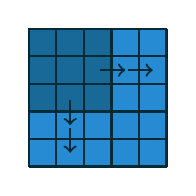
\begin{tikzpicture}[scale=.35,every node/.style={minimum size=1cm},
                            on grid]
            \draw[fill=blue] (0,0) rectangle (5,5);
            \draw[draw=base03, thick] (0,0) grid (5,5);
            \draw[fill=base02, opacity=0.4] (0,2) rectangle (3,5);
            \draw[step=10mm, base03, thick] (0,2) grid (3,5);
            \draw[draw=base03, ->, thick] (2.6,3.5) to  (3.5,3.5);
            \draw[draw=base03, ->, thick] (3.6,3.5) to  (4.5,3.5);
            \draw[draw=base03, ->, thick] (1.5,2.4) to  (1.5,1.5);
            \draw[draw=base03, ->, thick] (1.5,1.4) to  (1.5,0.5);
        \end{tikzpicture}
        \caption{\label{fig:no_padding_no_strides_explained} The kernel has to
            slide two steps to the right to touch the right side of the input
            (and equivalently downwards).  Adding one to account for the
            initial kernel position, the output size is $3 \times 3$.}
    \end{subfigure}
    ~
    \begin{subfigure}[t]{0.48\textwidth}
        \centering
        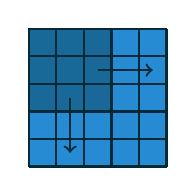
\begin{tikzpicture}[scale=.35,every node/.style={minimum size=1cm},
                            on grid]
            \draw[fill=blue] (0,0) rectangle (5,5);
            \draw[draw=base03, thick] (0,0) grid (5,5);
            \draw[fill=base02, opacity=0.4] (0,2) rectangle (3,5);
            \draw[step=10mm, base03, thick] (0,2) grid (3,5);
            \draw[draw=base03, ->, thick] (2.5,3.5) to  (4.5,3.5);
            \draw[draw=base03, ->, thick] (1.5,2.5) to  (1.5,0.5);
        \end{tikzpicture}
        \caption{\label{fig:no_padding_strides_explained} The kernel has to
            slide one step of size two to the right to touch the right side of
            the input (and equivalently downwards).  Adding one to account for
            the initial kernel position, the output size is $2 \times 2$.}
    \end{subfigure}
    \caption{Counting kernel positions.}
\end{figure}

\chapter{池化运算(Pooling arithmetic)}

In a neural network, pooling layers provide invariance to small translations of
the input. The most common kind of pooling is \emph{max pooling}, which
consists in splitting the input in (usually non-overlapping) patches and
outputting the maximum value of each patch. Other kinds of pooling exist, e.g.,
mean or average pooling, which all share the same idea of aggregating the input
locally by applying a non-linearity to the content of some patches \citep{%
boureau-cvpr-10,boureau-icml-10,boureau-iccv-11,ICML2011Saxe_551}.

Some readers may have noticed that the treatment of convolution arithmetic only
relies on the assumption that some function is repeatedly applied onto subsets
of the input. This means that the relationships derived in the previous chapter
can be reused in the case of pooling arithmetic. Since pooling does not involve
zero padding, the relationship describing the general case is as follows:

\begin{relationship}\label{rel:pooling}
For any $i$, $k$ and $s$,
\begin{equation*}
    o = \left\lfloor \frac{i - k}{s} \right\rfloor + 1.
\end{equation*}
\end{relationship}

\noindent This relationship holds for any type of pooling.

\chapter{转置卷积运算(Transposed convolution arithmetic)}

The need for transposed convolutions generally arises from the desire to use a
transformation going in the opposite direction of a normal convolution, i.e.,
from something that has the shape of the output of some convolution to
something that has the shape of its input while maintaining a connectivity
pattern that is compatible with said convolution. For instance, one might use
such a transformation as the decoding layer of a convolutional autoencoder or to
project feature maps to a higher-dimensional space.

Once again, the convolutional case is considerably more complex than the
fully-connected case, which only requires to use a weight matrix whose shape
has been transposed. However, since every convolution boils down to an
efficient implementation of a matrix operation, the insights gained from the
fully-connected case are useful in solving the convolutional case.

Like for convolution arithmetic, the dissertation about transposed convolution
arithmetic is simplified by the fact that transposed convolution properties
don't interact across axes.

The chapter will focus on the following setting:

\begin{itemize}
    \item 2-D transposed convolutions ($N = 2$),
    \item square inputs ($i_1 = i_2 = i$),
    \item square kernel size ($k_1 = k_2 = k$),
    \item same strides along both axes ($s_1 = s_2 = s$),
    \item same zero padding along both axes ($p_1 = p_2 = p$).
\end{itemize}

\noindent Once again, the results outlined generalize to the N-D and non-square
cases.

\section{作为矩阵运算的卷积}

Take for example the convolution represented in
\autoref{fig:no_padding_no_strides}. If the input and output were to be unrolled
into vectors from left to right, top to bottom, the convolution could be
represented as a sparse matrix $\mathbf{C}$ where the non-zero elements are the
elements $w_{i,j}$ of the kernel (with $i$ and $j$ being the row and column of
the kernel respectively):
\begin{equation*}
\resizebox{.98\hsize}{!}{$
    \begin{pmatrix}
    w_{0,0} & w_{0,1} & w_{0,2} & 0       & w_{1,0} & w_{1,1} & w_{1,2} & 0       &
    w_{2,0} & w_{2,1} & w_{2,2} & 0       & 0       & 0       & 0       & 0       \\
    0       & w_{0,0} & w_{0,1} & w_{0,2} & 0       & w_{1,0} & w_{1,1} & w_{1,2} &
    0       & w_{2,0} & w_{2,1} & w_{2,2} & 0       & 0       & 0       & 0       \\
    0       & 0       & 0       & 0       & w_{0,0} & w_{0,1} & w_{0,2} & 0       &
    w_{1,0} & w_{1,1} & w_{1,2} & 0       & w_{2,0} & w_{2,1} & w_{2,2} & 0       \\
    0       & 0       & 0       & 0       & 0       & w_{0,0} & w_{0,1} & w_{0,2} &
    0       & w_{1,0} & w_{1,1} & w_{1,2} & 0       & w_{2,0} & w_{2,1} & w_{2,2} \\
    \end{pmatrix}$}
\end{equation*}

This linear operation takes the input matrix flattened as a 16-dimensional
vector and produces a 4-dimensional vector that is later reshaped as the $2
\times 2$ output matrix.

Using this representation, the backward pass is easily obtained by transposing
$\mathbf{C}$; in other words, the error is backpropagated by multiplying the
loss with $\mathbf{C}^T$. This operation takes a 4-dimensional vector as input
and produces a 16-dimensional vector as output, and its connectivity pattern is
compatible with $\mathbf{C}$ by construction.

Notably, the kernel $\mathbf{w}$ defines both the matrices $\mathbf{C}$ and
$\mathbf{C}^T$ used for the forward and backward passes.

\section{转置卷积(Transposed convolution)}

Let's now consider what would be required to go the other way around, i.e., map
from a 4-dimensional space to a 16-dimensional space, while keeping the
connectivity pattern of the convolution depicted in
\autoref{fig:no_padding_no_strides}. This operation is known as a {\em
transposed convolution}.

Transposed convolutions -- also called {\em fractionally strided convolutions\/}
or {\em deconvolutions\/}\footnote{The term ``deconvolution'' is sometimes used
in the literature, but we advocate against it on the grounds that a
deconvolution is mathematically defined as the inverse of a convolution, which
is different from a transposed convolution.} -- work by swapping the forward and
backward passes of a convolution. One way to put it is to note that the kernel
defines a convolution, but whether it's a direct convolution or a transposed
convolution is determined by how the forward and backward passes are computed.

For instance, although the kernel $\mathbf{w}$ defines a convolution whose
forward and backward passes are computed by multiplying with $\mathbf{C}$ and
$\mathbf{C}^T$ respectively, it {\em also\/} defines a transposed convolution
whose forward and backward passes are computed by multiplying with
$\mathbf{C}^T$ and $(\mathbf{C}^T)^T = \mathbf{C}$ respectively.\footnote{The
    transposed convolution operation can be thought of as the gradient of {\em
    some\/} convolution with respect to its input, which is usually how
    transposed convolutions are implemented in practice.}

Finally note that it is always possible to emulate a transposed convolution with
a direct convolution. The disadvantage is that it usually involves adding many
columns and rows of zeros to the input, resulting in a much less efficient
implementation.

Building on what has been introduced so far, this chapter will proceed somewhat
backwards with respect to the convolution arithmetic chapter, deriving the
properties of each transposed convolution by referring to the direct
convolution with which it shares the kernel, and defining the equivalent direct
convolution.

\section{无零填充,单位步长,转置}

The simplest way to think about a transposed convolution on a given input is to
imagine such an input as being the result of a direct convolution applied on
some initial feature map. The trasposed convolution can be then considered as
the operation that allows to recover the \emph{shape}~\footnote{Note that the
  transposed convolution does not guarantee to recover the input itself, as it
  is not defined as the inverse of the convolution, but rather just returns a
  feature map that has the same width and height.} of this initial feature map.

Let's consider the convolution of a $3 \times 3$ kernel on a $4 \times 4$
input with unitary stride and no padding (i.e., $i = 4$, $k = 3$, $s = 1$ and
$p = 0$). As depicted in \autoref{fig:no_padding_no_strides}, this produces a
$2 \times 2$ output. The transpose of this convolution will then have an output
of shape $4 \times 4$ when applied on a $2 \times 2$ input.

Another way to obtain the result of a transposed convolution is to apply an
equivalent -- but much less efficient -- direct convolution. The example
described so far could be tackled by convolving a $3 \times 3$ kernel over a
$2 \times 2$ input padded with a $2 \times 2$ border of zeros using unit
strides (i.e., $i' = 2$, $k' = k$, $s' = 1$ and $p' = 2$), as shown in
\autoref{fig:no_padding_no_strides_transposed}. Notably, the kernel's and
stride's sizes remain the same, but the input of the transposed convolution is
now zero padded.\footnote{Note that although
    equivalent to applying the transposed matrix, this visualization adds a lot
    of zero multiplications in the form of zero padding.  This is done here for
    illustration purposes, but it is inefficient, and software implementations
    will normally not perform the useless zero multiplications.}

One way to understand the logic behind zero padding is to consider the
connectivity pattern of the transposed convolution and use it to guide the
design of the equivalent convolution. For example, the top left pixel of the
input of the direct convolution only contribute to the top left pixel of the
output, the top right pixel is only connected to the top right output pixel,
and so on.

To maintain the same connectivity pattern in the equivalent convolution it is
necessary to zero pad the input in such a way that the first (top-left)
application of the kernel only touches the top-left pixel, i.e., the padding
has to be equal to the size of the kernel minus one.

Proceeding in the same fashion it is possible to determine similar observations
for the other elements of the image, giving rise to the following relationship:

\begin{relationship}\label{rel:no_padding_no_strides_transposed}
A convolution described by $s = 1$, $p = 0$ and $k$ has an associated
transposed convolution described by $k' = k$, $s' = s$ and $p' = k - 1$ and its
output size is
\begin{equation*}
    o' = i' + (k - 1).
\end{equation*}
\end{relationship}

Interestingly, this corresponds to a fully padded convolution with unit
strides.

\section{Zero padding, unit strides, transposed}

Knowing that the transpose of a non-padded convolution is equivalent to
convolving a zero padded input, it would be reasonable to suppose that the
transpose of a zero padded convolution is equivalent to convolving an input
padded with {\em less\/} zeros.

It is indeed the case, as shown in
\autoref{fig:arbitrary_padding_no_strides_transposed} for $i = 5$, $k = 4$ and
$p = 2$.

Formally, the following relationship applies for zero padded convolutions:

\begin{relationship}\label{rel:arbitrary_padding_no_strides_transposed}
A convolution described by $s = 1$, $k$ and $p$ has an
associated transposed convolution described by $k' = k$, $s' = s$ and $p' = k -
p - 1$ and its output size is
\begin{equation*}
    o' = i' + (k - 1) - 2p.
\end{equation*}
\end{relationship}

\begin{figure}[p]
    \centering
    \includegraphics[width=0.24\textwidth]{pdf/no_padding_no_strides_transposed_00.pdf}
    \includegraphics[width=0.24\textwidth]{pdf/no_padding_no_strides_transposed_01.pdf}
    \includegraphics[width=0.24\textwidth]{pdf/no_padding_no_strides_transposed_02.pdf}
    \includegraphics[width=0.24\textwidth]{pdf/no_padding_no_strides_transposed_03.pdf}
    \caption{\label{fig:no_padding_no_strides_transposed} The transpose of
        convolving a $3 \times 3$ kernel over a $4 \times 4$ input using unit
        strides (i.e., $i = 4$, $k = 3$, $s = 1$ and $p = 0$). It is equivalent
        to convolving a $3 \times 3$ kernel over a $2 \times 2$ input padded
        with a $2 \times 2$ border of zeros using unit strides (i.e., $i' = 2$,
        $k' = k$, $s' = 1$ and $p' = 2$).}
\end{figure}

\begin{figure}[p]
    \centering
    \includegraphics[width=0.24\textwidth]{pdf/arbitrary_padding_no_strides_transposed_00.pdf}
    \includegraphics[width=0.24\textwidth]{pdf/arbitrary_padding_no_strides_transposed_01.pdf}
    \includegraphics[width=0.24\textwidth]{pdf/arbitrary_padding_no_strides_transposed_02.pdf}
    \includegraphics[width=0.24\textwidth]{pdf/arbitrary_padding_no_strides_transposed_03.pdf}
    \caption{\label{fig:arbitrary_padding_no_strides_transposed} The transpose
        of convolving a $4 \times 4$ kernel over a $5 \times 5$ input padded
        with a $2 \times 2$ border of zeros using unit strides (i.e., $i = 5$,
        $k = 4$, $s = 1$ and $p = 2$). It is equivalent to convolving a $4
        \times 4$ kernel over a $6 \times 6$ input padded with a $1 \times 1$
        border of zeros using unit strides (i.e., $i' = 6$, $k' = k$, $s' = 1$
        and $p' = 1$).}
\end{figure}

\begin{figure}[p]
    \centering
    \includegraphics[width=0.24\textwidth]{pdf/same_padding_no_strides_transposed_00.pdf}
    \includegraphics[width=0.24\textwidth]{pdf/same_padding_no_strides_transposed_01.pdf}
    \includegraphics[width=0.24\textwidth]{pdf/same_padding_no_strides_transposed_02.pdf}
    \includegraphics[width=0.24\textwidth]{pdf/same_padding_no_strides_transposed_03.pdf}
    \caption{\label{fig:same_padding_no_strides_transposed} The transpose of
        convolving a $3 \times 3$ kernel over a $5 \times 5$ input using half
        padding and unit strides (i.e., $i = 5$, $k = 3$, $s = 1$ and $p = 1$).
        It is equivalent to convolving a $3 \times 3$ kernel over a $5 \times 5$
        input using half padding and unit strides (i.e., $i' = 5$, $k' = k$, $s'
        = 1$ and $p' = 1$).}
\end{figure}

\subsection{Half (same) padding, transposed}

By applying the same inductive reasoning as before, it is reasonable to expect
that the equivalent convolution of the transpose of a half padded convolution
is itself a half padded convolution, given that the output size of a half
padded convolution is the same as its input size. Thus the following relation
applies:

\begin{relationship}\label{rel:half_padding_no_strides_transposed}
A convolution described by $k = 2n + 1, \quad n \in \mathbb{N}$, $s = 1$ and $p
= \lfloor k / 2 \rfloor = n$ has an associated transposed convolution described
by $k' = k$, $s' = s$ and $p' = p$ and its output size is
\begin{equation*}
\begin{split}
    o' &= i' + (k - 1) - 2p \\
       &= i' + 2n - 2n \\
       &= i'.
\end{split}
\end{equation*}
\end{relationship}

\autoref{fig:same_padding_no_strides_transposed} provides an example for $i =
5$, $k = 3$ and (therefore) $p = 1$.

\subsection{Full padding, transposed}

Knowing that the equivalent convolution of the transpose of a non-padded
convolution involves full padding, it is unsurprising that the equivalent of
the transpose of a fully padded convolution is a non-padded convolution:

\begin{relationship}\label{rel:full_padding_no_strides_transposed}
A convolution described by $s = 1$, $k$ and $p = k - 1$ has an
associated transposed convolution described by $k' = k$, $s' = s$ and $p' = 0$
and its output size is
\begin{equation*}
\begin{split}
    o' &= i' + (k - 1) - 2p \\
       &= i' - (k - 1)
\end{split}
\end{equation*}
\end{relationship}

\autoref{fig:full_padding_no_strides_transposed} provides an example for $i =
5$, $k = 3$ and (therefore) $p = 2$.

\section{No zero padding, non-unit strides, transposed}

Using the same kind of inductive logic as for zero padded convolutions, one
might expect that the transpose of a convolution with $s > 1$ involves an
equivalent convolution with $s < 1$. As will be explained, this is a valid
intuition, which is why transposed convolutions are sometimes called {\em
fractionally strided convolutions}.

\autoref{fig:no_padding_strides_transposed} provides an example for $i = 5$, $k
= 3$ and $s = 2$ which helps understand what fractional strides involve: zeros
are inserted {\em between\/} input units, which makes the kernel move around at
a slower pace than with unit strides.\footnote{Doing so is inefficient and
    real-world implementations avoid useless multiplications by zero, but
    conceptually it is how the transpose of a strided convolution can be
    thought of.}

For the moment, it will be assumed that the convolution is non-padded ($p = 0$)
and that its input size $i$ is such that $i - k$ is a multiple of $s$. In that
case, the following relationship holds:

\begin{relationship}\label{rel:no_padding_strides_transposed}
A convolution described by $p = 0$, $k$ and $s$ and whose input
size is such that $i - k$ is a multiple of $s$, has an associated transposed
convolution described by $\tilde{i}'$, $k' = k$, $s' = 1$ and $p' = k - 1$,
where $\tilde{i}'$ is the size of the stretched input obtained by adding
$s - 1$ zeros between each input unit, and its output size is
\begin{equation*}
\begin{split}
    o' = s (i' - 1) + k.
\end{split}
\end{equation*}
\end{relationship}

\begin{figure}[p]
    \centering
    \includegraphics[width=0.24\textwidth]{pdf/full_padding_no_strides_transposed_00.pdf}
    \includegraphics[width=0.24\textwidth]{pdf/full_padding_no_strides_transposed_01.pdf}
    \includegraphics[width=0.24\textwidth]{pdf/full_padding_no_strides_transposed_02.pdf}
    \includegraphics[width=0.24\textwidth]{pdf/full_padding_no_strides_transposed_03.pdf}
    \caption{\label{fig:full_padding_no_strides_transposed} The transpose of
        convolving a $3 \times 3$ kernel over a $5 \times 5$ input using full
        padding and unit strides (i.e., $i = 5$, $k = 3$, $s = 1$ and $p = 2$).
        It is equivalent to convolving a $3 \times 3$ kernel over a $7 \times 7$
        input using unit strides (i.e., $i' = 7$, $k' = k$, $s' = 1$ and $p' =
        0$).}
\end{figure}

\begin{figure}[p]
    \centering
    \includegraphics[width=0.24\textwidth]{pdf/no_padding_strides_transposed_00.pdf}
    \includegraphics[width=0.24\textwidth]{pdf/no_padding_strides_transposed_01.pdf}
    \includegraphics[width=0.24\textwidth]{pdf/no_padding_strides_transposed_02.pdf}
    \includegraphics[width=0.24\textwidth]{pdf/no_padding_strides_transposed_03.pdf}
    \caption{\label{fig:no_padding_strides_transposed} The transpose of
        convolving a $3 \times 3$ kernel over a $5 \times 5$ input using $2
        \times 2$ strides (i.e., $i = 5$, $k = 3$, $s = 2$ and $p = 0$). It is
        equivalent to convolving a $3 \times 3$ kernel over a $2 \times 2$ input
        (with $1$ zero inserted between inputs) padded with a $2 \times 2$
        border of zeros using unit strides (i.e., $i' = 2$, $\tilde{i}' = 3$, $k'
        = k$, $s' = 1$ and $p' = 2$).}
\end{figure}

\begin{figure}[p]
    \centering
    \includegraphics[width=0.24\textwidth]{pdf/padding_strides_transposed_00.pdf}
    \includegraphics[width=0.24\textwidth]{pdf/padding_strides_transposed_01.pdf}
    \includegraphics[width=0.24\textwidth]{pdf/padding_strides_transposed_02.pdf}
    \includegraphics[width=0.24\textwidth]{pdf/padding_strides_transposed_03.pdf}
    \caption{\label{fig:padding_strides_transposed} The transpose of convolving
        a $3 \times 3$ kernel over a $5 \times 5$ input padded with a $1 \times
        1$ border of zeros using $2 \times 2$ strides (i.e., $i = 5$, $k = 3$, $s
        = 2$ and $p = 1$). It is equivalent to convolving a $3 \times 3$ kernel
        over a $3 \times 3$ input (with $1$ zero inserted between inputs) padded
        with a $1 \times 1$ border of zeros using unit strides (i.e., $i' = 3$,
        $\tilde{i}' = 5$, $k' = k$, $s' = 1$ and $p' = 1$).}
\end{figure}

\section{Zero padding, non-unit strides, transposed}

When the convolution's input size $i$ is such that $i + 2p - k$ is a multiple
of $s$, the analysis can extended to the zero padded case by combining
\autoref{rel:arbitrary_padding_no_strides_transposed} and
\autoref{rel:no_padding_strides_transposed}:

\begin{relationship}\label{rel:padding_strides_transposed}
A convolution described by $k$, $s$ and $p$ and whose
input size $i$ is such that $i + 2p - k$ is a multiple of $s$ has an associated
transposed convolution described by $\tilde{i}'$, $k' = k$, $s' = 1$ and
$p' = k - p - 1$, where $\tilde{i}'$ is the size of the stretched input
obtained by adding $s - 1$ zeros between each input unit, and its output size
is
\begin{equation*}
\begin{split}
    o' = s (i' - 1) + k - 2p.
\end{split}
\end{equation*}
\end{relationship}

\autoref{fig:padding_strides_transposed} provides an example for $i = 5$, $k =
3$, $s = 2$ and $p = 1$.

The constraint on the size of the input $i$ can be relaxed by introducing
another parameter $a \in \{0, \ldots, s - 1\}$ that allows to distinguish
between the $s$ different cases that all lead to the same $i'$:

\begin{relationship}\label{rel:padding_strides_transposed_odd}
A convolution described by $k$, $s$ and $p$ has an
associated transposed convolution described by $a$, $\tilde{i}'$, $k' = k$, $s'
= 1$ and $p' = k - p - 1$, where $\tilde{i}'$ is the size of the stretched
input obtained by adding $s - 1$ zeros between each input unit, and $a = (i +
2p - k) \mod s$ represents the number of zeros added to the bottom and right edges
of the input, and its output size is
\begin{equation*}
\begin{split}
    o' = s (i' - 1) + a + k - 2p.
\end{split}
\end{equation*}
\end{relationship}

\autoref{fig:padding_strides_odd_transposed} provides an example for $i = 6$, $k
= 3$, $s = 2$ and $p = 1$.

\begin{figure}[p]
    \centering
    \includegraphics[width=0.24\textwidth]{pdf/padding_strides_odd_transposed_00.pdf}
    \includegraphics[width=0.24\textwidth]{pdf/padding_strides_odd_transposed_01.pdf}
    \includegraphics[width=0.24\textwidth]{pdf/padding_strides_odd_transposed_02.pdf}
    \includegraphics[width=0.24\textwidth]{pdf/padding_strides_odd_transposed_03.pdf}
    \caption{\label{fig:padding_strides_odd_transposed} The transpose of
        convolving a $3 \times 3$ kernel over a $6 \times 6$ input padded with a
        $1 \times 1$ border of zeros using $2 \times 2$ strides (i.e., $i = 6$,
        $k = 3$, $s = 2$ and $p = 1$). It is equivalent to convolving a $3
        \times 3$ kernel over a $2 \times 2$ input (with $1$ zero inserted
        between inputs) padded with a $1 \times 1$ border of zeros (with an
        additional border of size $1$ added to the bottom and right edges) using
        unit strides (i.e., $i' = 3$, $\tilde{i}' = 5$, $a = 1$, $k' = k$, $s' =
        1$ and $p' = 1$).}
\end{figure}

\chapter{其他卷积(Miscellaneous convolutions)}

\section{扩张卷积(Dilated convolutions)}

Readers familiar with the deep learning literature may have noticed the term
``dilated convolutions'' (or ``atrous convolutions'', from the French expression
{\em convolutions \`{a} trous}) appear in recent papers. Here we attempt to
provide an intuitive understanding of dilated convolutions. For a more in-depth
description and to understand in what contexts they are applied, see
\citet{chen2014semantic,yu2015multi}.

Dilated convolutions ``inflate'' the kernel by inserting spaces between the
kernel elements. The dilation ``rate'' is controlled by an additional
hyperparameter $d$. Implementations may vary, but there are usually $d - 1$
spaces inserted between kernel elements such that $d = 1$ corresponds to a
regular convolution.

Dilated convolutions are used to cheaply increase the receptive field of output
units without increasing the kernel size, which is especially effective
when multiple dilated convolutions are stacked one after another. For a
concrete example, see \citet{oord2016wavenet}, in which the proposed WaveNet
model implements an autoregressive generative model for raw audio which uses
dilated convolutions to condition new audio frames on a large context of past
audio frames.

To understand the relationship tying the dilation rate $d$ and the output size
$o$, it is useful to think of the impact of $d$ on the {\em effective kernel
size}. A kernel of size $k$ dilated by a factor $d$ has an effective size
\begin{equation*}
    \hat{k} = k + (k - 1)(d - 1).
\end{equation*}
This can be combined with \autoref{rel:padding_strides} to form the following
relationship for dilated convolutions:

\begin{relationship}\label{rel:dilation}
For any $i$, $k$, $p$ and $s$, and for a dilation rate $d$,
\begin{equation*}
    o = \left\lfloor \frac{i + 2p - k - (k - 1)(d - 1)}{s} \right\rfloor + 1.
\end{equation*}
\end{relationship}

\begin{figure}[h]
    \centering
    \includegraphics[width=0.24\textwidth]{pdf/dilation_00.pdf}
    \includegraphics[width=0.24\textwidth]{pdf/dilation_01.pdf}
    \includegraphics[width=0.24\textwidth]{pdf/dilation_02.pdf}
    \includegraphics[width=0.24\textwidth]{pdf/dilation_03.pdf}
    \caption{\label{fig:dilation} (Dilated convolution)
        Convolving a $3 \times 3$ kernel over a $7 \times 7$ input with a
        dilation factor of 2 (i.e., $i = 7$, $k = 3$, $d = 2$, $s = 1$ and
        $p = 0$).}
\end{figure}

\noindent \autoref{fig:dilation} provides an example for $i = 7$, $k = 3$ and
$d = 2$.

\bibliography{bibliography}
\bibliographystyle{natbib}
\end{document}
